\documentclass{llncs}
%
\usepackage{url}
\RequirePackage[hyphenbreaks]{breakurl} % allow hyphenation in URLs
\usepackage{amsmath} % use equations
\RequirePackage[utf8]{inputenc} % support Umlauts and special characters
\usepackage{microtype} % use space more efficiently and hyphenate smarter: all in all looks a lot sexier
\usepackage{listings} % allow source code environments
\usepackage{graphicx}

%
\title{Jadex}
\subtitle{An agent framework}
\titlerunning{agentprog}
\author{Manuel Mittler}
\institute{University Koblenz-Landau}
\tocauthor{ }
%
\begin{document}
\maketitle
\tableofcontents

\section{Introduction}
Nowadays a couple of agent frameworks is available for developing multi-agent applications. \cite{Mangina} Jadex focuses on the development of goal-oriented agents following the belief-desire-intention (BDI) model. It aims at bringing middleware and reasoning-centred agent platforms together. For that purpose Jadex uses the Java agent development framework (JADE) as a middleware and puts on top of that a rational reasoning engine. Jadex integrates agent-theories with object-orientation and XML descriptions. No new programming language is introduced. 
\begin{figure}
	\centering
	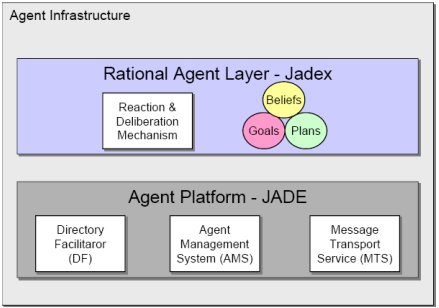
\includegraphics{Jadex_infrastructure.png}
	\caption{Jadex Infrastrucuture}
	\label{fig1}
\end{figure}
JADE is also a Java framework that provides communication infrastructure, platform services such as agent management und a set of development and debugging tools. It enables the development and execution of  peer-to-peer applications which are based on the agent paradigm (autonomous, proactive and social). The agents are identified by a unique name and provide a set of 
services. They can register and modify their services 
and/or search for agents providing given services (white and yellow pages). Additionally they are capable of controlling their life cycle and they can dynamically discover other agents and communicate 
with them: exchange asynchronous messages via an agent communication language (ACL)). 

\section{Architecture}
This section presents the architecture of Jadex. "`Viewed from the outside, an agent is a black box, which receives and sends messages."' \cite{Pokahr} (see figure 2)
\begin{figure}
	\centering
	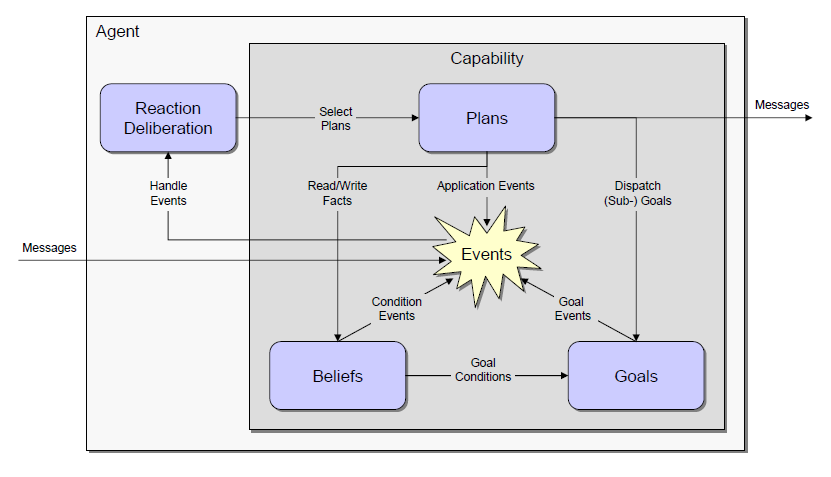
\includegraphics[width=300px]{Jadex_agent.png}
	\caption{Jadex abstract agent \cite{Pokahr}}
	\label{fig2}
\end{figure}
Beliefs are single facts stored as Java objects which represent the knowledge of an agent. They are stored as key-value pairs. The advantage of storing information as facts is that the programmer has a central place for the knowledge und can query the agent's beliefs. Monitoring of the beliefs is possible, too. 
The goals are momentary desires of an agent for which the agent engages into suitable actions until it considers the goal as being reached, unreachable, or not wanted anymore. Jadex distinguishes between four generic goal types. A perform goal is directly related to the execution of actions. Therefore, the goal is considered to be reached, when some actions have been executed, regardless of the outcome of these actions. An achieve goal is a goal in the traditional sense, which defines a desired world state without specifying how to reach it. Agents may try several different alternative plans, to achieve a goal of this type. A query goal is similar to an achieve goal, but the desired state is not a state of the (outside) world, but in internal state of the agent, regarding the availability of some information the agent wants to know about. For goals of type maintain an agents keep track of a desired state, and will continously execute appropriate plans to re-establish this maintained state whenever needed. In contrast to goals, events are (per default) dispatched to all interested plans but do not support any BDI-mechanism. Therefore the originator of an internal event is usually not interested in the effect the internal event may produce but only wants to inform some interested parties about some occurrence. Plans represent the behavioral elements of an agent and are composed of a head and a body part. The plan head specification is similar to other BDI systems and mainly specifies the circumstances under which a plan may be selected, e.g. by stating events or goals handled by the plan and preconditions for the execution of the plan. Additionally, in the plan head a context condition can be stated that must be true for the plan to continue executing. The plan body provides a predefined course of action, given in a procedural language. This course of action is to be executed by the agent, when the plan is selected for execution, and may contain actions provided by the system API, such as sending messages, manipulating beliefs, or creating subgoals. (cf \cite{Pokahr2})

\section{Components of a Jadex agent}
Jadex is not based on a new agent programming language. Instead, a hybrid approach is chosen, distinguishing explicitly between the language used for static agent type specification and the language for defining the dynamic agent behavior. An agent in Jadex consists of two components: An agent defintion file (ADF) for the specification of beliefs, goals, and plans as well as their initial values and on the other hand procedural plan code. The procedural part of plans  (the plan bodies) are realized in an ordinary programming language (Java) and have access to the BDI facilities of an agent through an application interface (API). The plan body is a standard Java class that extends a predifined Jadex framework class and has at least to implement the abstract body() method which is invoked after plan instantiation. The plan body is associated to a plan head in the ADF. This means that in the plan head several properties of the plan can be specified, e.g. the circumstances under which it is activated and its importance in relation to other plans. There are two types of plans in Jadex. A service plan and a passive plan. The service plan, as the name indicates, is an instance of a plan which waits for service requests. Therefore a service plan  can setup its private event waitqueue and receive events for later processing, even when it is working at the moment. In contrast to that, a passive plan is only running when it has a task to achieve. For this kind of plan the triggering event and goals must be specified must be specified in the agent defenition file to let the agent know what kinds of events this plan can handle. When an agent receives an event, the BDI reasoning engine builds up the so called applicable plan list which contains all plans that can handle the current event or goal. The candidates are selected and istantiated for execution.

\section{Execution model}
The execution model for Jadex looks like the following:
\begin{figure}
	\centering
	\includegraphics[width=300px]{execution_model.png}
	\label{fig3}
	\caption{Jadex execution model \cite{Pokahr}}
\end{figure}
\newline
When an agent recieves a message it is placed at a message queue. In the next step the message has to be assigned to a capability, which can handle the message. A suitable capability is found by matching the message against the event templates defined in the eventbase of each capability. The best matching template is then used to create an appropriate event in the scope of the capability. After that the created event is subsequently added to the agent's global event list. The dispatcher is responsible for selecting applicable plans for the events from the event list. After plans have been selected, they are placed in the ready list, waiting for execution. The execution of plans is performed by a scheduler, which selects plans from the ready list. 

\section{Conclusion}
All in all Jadex is a very powerfull tool that supports easy agent construction with XML-based agent description and procedural plans in Java. Additionally it offers tool support for development debugging. It comes for example with a BDI-Viewer that allows observing and modifying the internal state of an agent and a logger agent that collects log-outputs of any agent. The author considers that Jadex is suitable for the purpose of competing in the multi agent programming contest. Extensive documentation, tutorials and user guides can be found on the website of the developers \cite{Jadex}.

\newpage
\bibliographystyle{splncs03}

\bibliography{sources_jadex}
\end{document}
